% !TEX root = ../thesis.tex

\chapter{Einleitung und Motivation}
\label{introduction}

Softwarefehler stellen einen erheblichen Auslöser für finanzielle Schäden und Rufschädigungen von Unternehmen dar. Solche Fehler reichen von kleineren \glqq Bugs\grqq{} bis hin zu schwerwiegenden Sicherheitslücken. Aus diesem Grund herrscht ein großes Interesse daran, einen Entwickler zu warnen, wenn er aktualisierten Softwarecode veröffentlicht, der möglicherweise einen oder mehrere Fehler beinhaltet. 

Zu diesem Zweck haben Forscher und Softwareentwickler im vergangenen Jahrzehnt verschiedene Techniken zur Fehlererkennung und Fehlervorhersage entwickelt, die zu einem Großteil auf Methoden und Techniken des \emph{Machine Learnings} basieren \cite{Challagulla2008}. Diese verwenden in der Regel historische Daten von fehlerhaften und fehlerfreien Änderungen an Softwaresystemen in Kombination mit einer sorgfältig zusammengestellten Menge von \emph{Attributen} (in der Regel Features genannt\footnote{Um einem missverständlichen und doppeldeutigen Gebrauch des Feature-Begriffes vorzubeugen, wird für die hier verwendete Beschreibung der Charakteristika von Daten auch im weiteren Verlauf dieser Ausarbeitung der Begriff \glqq Attribute\grqq{} verwendet.}), um einen gegebenen Klassifikator zu trainieren \cite{Alsaeedi2019,Hammouri2018}. Dieser kann dann anschließend verwendet werden, um eine akkurate Vorhersage zu erhalten, ob eine neu erfolgte Änderung an einer Software fehlerhaft oder frei von Fehlern ist.

Die Auswahl an Algorithmen für die Klassifikation ist groß. Studien zeigen, dass aus dem Pool von verfügbaren Algorithmen sowohl Entscheidungsbaum-basierte (zum Beispiel J48, CART oder Random Forest) als auch Bayessche Algorithmen (zum Beispiel Na\"{\i}ve Bayes (NB), Bernoulli-NB oder multinomieller NB) die meistgenutzten sind \cite{Son2019}. Alternative Algorithmen sind beispielsweise Regression, k-Nearest-Neighbors oder künstliche neuronale Netze \cite{Challagulla2008}. Anzumerken ist allerdings, dass es keinen Konsens über den besten verfügbaren Algorithmus gibt, da jeder Algorithmus unterschiedliche Stärken und Schwächen für bestimmte Anwendungsfälle aufweist.

Das Ziel dieser Arbeit ist die Entwicklung einer solchen Vorhersagetechnik für Softwarefehler basierend auf Software-Features. Diese Features beschreiben Inkremente der Funktionalität eines Softwaresystems. Die auf diese Weise entwickelten Softwaresysteme heißen Software-Produktlinien und bestehen aus einer Menge von ähnlichen Softwareprodukten. Sie zeichnen sich dadurch aus, dass sie eine gemeinsame Menge von Features sowie eine gemeinsame Codebasis besitzen \cite{Thuem2014}. Durch das Vorhandensein verschiedener Features entlang der Softwareprodukte, kann eine breite Variabilität innerhalb einer Produktlinie erreicht werden. Eine detaillierte Einführung in den Themenkomplex von Software-Produktlinien und featurebasierter Softwareentwicklung kann in \hyperref[feat-develop]{Abschnitt 2.1} gefunden werden. Bei der Entwicklung der Vorhersagetechnik wird die Implementation von Features mittels Präprozessor-Anweisungen, wie \texttt{\#IFDEF} und \texttt{\#IFNDEF} (auch Präprozessor-Direktiven genannt) betrachtet. Dieser bisher in wissenschaftlichen Arbeiten nur einmal im Rahmen einer Fallstudie betrachtete Ansatz \cite{Queiroz2016} ist aufgrund mehrerer Gründe chancenreich:

\begin{enumerate}
\setlength{\itemsep}{-2pt}
\item Wenn ein bestimmtes Feature in der Vergangenheit mehr oder weniger fehleranfällig war, so ist eine Änderung, die das Feature aktualisiert, wahrscheinlich ebenfalls mehr oder weniger fehleranfällig. 
\item Features, die mehr oder weniger fehleranfällig scheinen, könnten besondere Eigenschaften haben, die im Rahmen der Fehlervorhersage verwendet werden können.
\item Code, der viel featuresspezifischen Code enthält (insbesondere die sogenannten Feature-Interaktionen), ist möglicherweise fehleranfälliger als sonstiger Code.
\end{enumerate}

Ein initiales und einfaches Beispiel für einen Softwarefehler innerhalb eines Features ist in \autoref{bug-code} dargestellt. Es ist zu erkennen, dass innerhalb des Codes des Features \texttt{print\_time} die \texttt{printf}-Anweisung einen Schreibfehler enthält, der dazu führt, dass der Featurecode nicht ausgeführt werden kann. Ferner kann fehlerhafter Featurecode dazu führen, dass die gesamte Funktionalität des Features und gegebenenfalls der gesamten Software beeinträchtigt oder verhindert wird. Ein reales Beispiel für einen Fehler aus dem Sourcecode des Softwareprojekts Vim ist in \autoref{fig:bug-example} dargestellt.

\begin{lstlisting}[language=Python, caption=Exemplarische Darstellung eines fehlerhaften Features, frame=single, label=bug-code]
int test() {
	  #IFDEF print_time
	  prntf("Current time: %s", time(&now));
	  #ENDIF

	  printf("Hello World!");
	  return 0;
  }
\end{lstlisting}
 
Das zuvor genannte Ziel der Arbeit setzt sich aus mehreren Teilzielen zusammen. Dazu zählen die Erstellung eines Datensets unter Einbezug des Feature-Aspekts (\hyperref[dataset-creation]{Kapitel 3}). Dieses Datenset dient wiederum zum Training einer repräsentativen Auswahl an Klassifikatoren (\hyperref[training]{Kapitel 4}) mit anschließender vergleichender Evaluation (\hyperref[evaluation]{Kapitel 5}) dieser. Zusätzlich wird das featurebasierte Datenset mit einem klassischen dateibasierten Datenset (\hyperref[classic-eval]{Abschnitt 5.3}) verglichen, dessen Entwicklung aus einer wissenschaftlichen Arbeit entnommen wurde \cite{Moser2008}. Ein genauer Überblick über die Forschungsziele befindet sich im nächsten Abschnitt.

Sollte sich im Rahmen der Evaluation einer dieser Klassifikatoren als besonders effektiv erweisen, so würde diese Arbeit den Stand der Technik hinsichtlich der Fehlererkennung in Features vorantreiben und Organisationen erlauben, bessere Einblicke in die Fehleranfälligkeit von Änderungen in ihrer durch Variabilität geprägten Codebasis zu erhalten.

\section{Forschungsziele und Forschungsfragen}

Wie bereits in der Einleitung beschrieben, ist das übergeordnete Ziel dieser Arbeit die Entwicklung einer Vorhersagetechnik für Fehler in featurebasierter Software unter Zuhilfenahme von Methoden des Machine Learnings. Dazu ist vorgesehen, das Augenmerk hinsichtlich der Datengrundlage auf Commits des Versionierungssystems Git zu richten. Ein Commit beschreibt dabei die Freischaltung von Veränderungen an einer oder mehreren Dateien. Als Datenbasis für das Trainieren der Klassifikatoren dienen dann Commits, für die auf Grundlage eines automatisierten Verfahrens aus der Literatur eine Klassifikation in \glqq defekt\grqq{} und \glqq fehlerfrei{}\grqq verfügbar ist. Dies ermöglicht es, für ausstehende oder zukünftige Softwareversionen akkurate Vorhersagen zu treffen, ob diese Fehler beinhalten. So kann das Risiko der Konsequenzen von Softwarefehlern gesenkt werden.

Der Prozess der Entwicklung der Vorhersagetechnik ist in drei zu erreichende Forschungsziele eingeteilt. Jedem Forschungsziel werden Forschungsfragen zugeordnet, deren Aufklärung einen zusätzlichen Teil zur Erfüllung der Ziele beiträgt. Im Folgenden werden die Forschungsziele (RO – \glqq research objective\grqq) mit ihren zugehörigen Forschungsfragen (RQ – \glqq research question\grqq) vorgestellt. Die Beantwortung der Forschungsfragen erfolgt im weiteren Verlauf der Arbeit. Erkennbar sind die Antworten auf die Fragen an ihrer Einrahmung.

\label{research_objectives}

\fbox{\parbox{\linewidth}{RO1: Erstellung eines Datensets zum Trainieren von relevanten Machine-Learning-Klassifikatoren
\begin{itemize}
 \renewcommand{\labelitemi}{$\Rightarrow$}
 \setlength{\itemsep}{-2pt}
 \item RQ1a: Welche Daten kommen für die Erstellung des Datensets in Frage?
 \item RQ1b: Wie weit müssen die Daten vorverarbeitet werden, um sie für das Training nutzbar zu machen?
\end{itemize}}}

\fbox{\parbox{\linewidth}{RO2: Identifikation und Training einer Auswahl von relevanten Machine-Learning-Klassifikatoren basierend auf dem Datenset
\begin{itemize}
 \renewcommand{\labelitemi}{$\Rightarrow$}
 \setlength{\itemsep}{-2pt}
 \item RQ2: Welche Machine-Learning-Klassifikatoren kommen für die gegebene Aufgabe in Frage?
\end{itemize}}}

\fbox{\parbox{\linewidth}{RO3: Evaluation und Gegenüberstellung der Klassifikatoren sowie Vergleich zu modernen Vorhersagetechniken, die keine Features nutzen
\begin{itemize}
 \renewcommand{\labelitemi}{$\Rightarrow$}
 \setlength{\itemsep}{-2pt}
 \item RQ3a: Welche miteinander vergleichbaren Merkmale besitzen die Klassifikatoren?
 \item RQ3b: Welche Metriken können für den Vergleich verwendet werden?
 \item RQ3c: Wie lassen sich die Klassifikatoren mit weiteren Vorhersagetechniken, die keine Features nutzen, vergleichen?
 \item RQ3d: Wie beeinflusst die Verwendung von featurebasierten Metriken die Fehlervorhersage?
\end{itemize}}}

\label{phases_definition}

Zusätzlich zu den drei genannten Forschungszielen umfasst die Bearbeitung der Masterarbeit eine Vor- und Nachbereitung, sodass sich insgesamt fünf Arbeitsphasen ergeben:

\begin{itemize}
\setlength{\itemsep}{-2pt}
\item Vorbereitung
\item Abschluss des ersten Forschungsziels (\textit{Erstellung des Datensets})
\item Abschluss des zweiten Forschungsziels (\textit{Training von Machine-Learning-Klassifikatoren})
\item Abschluss des dritten Forschungsziels (\textit{Evaluation und Vergleich})
\item Nachbereitung
\end{itemize}

Diese Arbeitsphasen werden im kommenden Abschnitt anhand des verwendeten Forschungsdesigns näher erläutert.
%Als finale Vorhersagetechnik wird jener Klassifikator verwendet, der sich im Rahmen der Gegenüberstellung im Verlauf der Evaluation als am \glqq effektivsten\grqq{} erweist. Die Kriterien für die Beurteilung der Effektivität eines Klassifikators werden im Kapitel \glqq \hyperref[evaluation]{Evaluation}\grqq{} erläutert.

\section{Forschungsdesign}

Die für diese Arbeit gewählte Methodik basiert auf dem Prozessmodell \glqq Cross-Industry Standard Process for Data Mining\grqq, kurz CRISP-DM, nach Chapman et al. \cite{Chapman2000}. Es wird als Vorlage für die Arbeitsphasen zur Erreichung der Forschungsziele dieser Arbeit verwendet. Da sich der überwiegende praktische Teil dieser Arbeit auf Programmierung im Bereich des Machine Learning konzentriert, bildet das CRISP-DM Prozessmodell ein passendes vordefiniertes Vorgehen. Eine grafische Aufarbeitung des Prozessmodells mit seinen sechs zugehörigen Phasen sowie den Verbindungen zwischen ihnen ist in \autoref{fig:crisp1} dargestellt. 

\begin{figure}[ht]
    \centering
    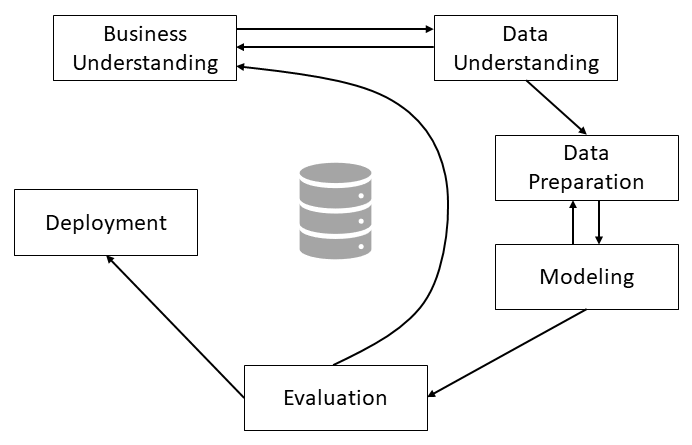
\includegraphics[width=0.6\textwidth]{images/CRISP-DM1}
    \caption{CRISP-DM Prozessmodell nach \cite{Chapman2000}}\label{fig:crisp1}
\end{figure}

Das CRISP-DM-Prozessmodell wurde, wie der ausgeschriebene Name bereits andeutet, ursprünglich für die Erarbeitung von Data-Mining-Projekten entwickelt, eignet sich jedoch auch zur Verwendung im Rahmen eines Machine Learning Projektes, da sich die in beiden Bereichen verwendeten Methoden und Prozesse zu einem erheblichen Teil überlagern. Ein Überblick über die sechs Phasen des Prozessmodells ist in \autoref{fig:crisp} dargestellt. Zusätzlich umfasst diese Abbildung die Zuordnung der Arbeitsphasen, die im \hyperref[phases_definition]{vorherigen Abschnitt} definiert wurden. Eine Erläuterung der Phasen des Prozessmodells erfolgt im Anschluss. 

\begin{figure}[ht]
    \centering
    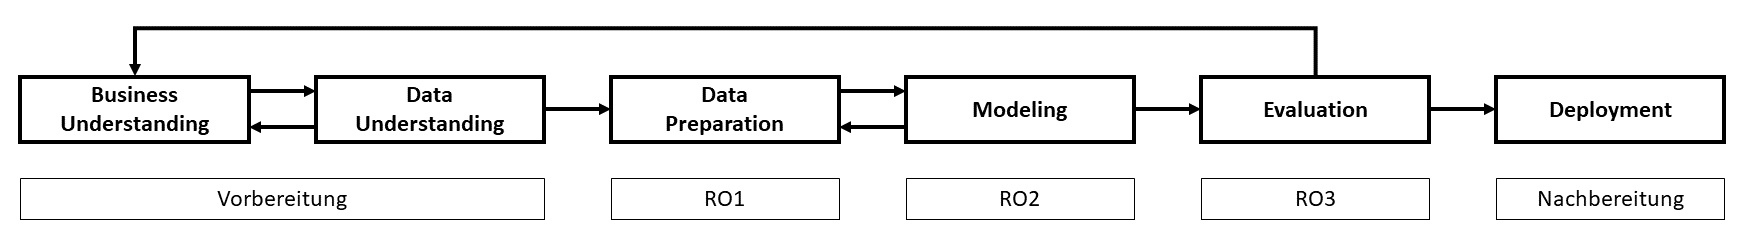
\includegraphics[width=\textwidth]{images/CRISP-DM}
    \caption{Phasen des CRISP-DM Prozessmodells nach \cite{Chapman2000} mit Zuordnung der Arbeitsphasen}\label{fig:crisp}
\end{figure}

Die ersten beiden Phasen \emph{Business Understanding} und \emph{Data Understanding} widmen sich der Vorbereitung der Arbeit. Die initiale Phase umfasst dabei die allgemeine Einarbeitung in das zugrundeliegende Thema und der Formulierung der Forschungsziele. Die darauffolgende Phase \emph{Data Understanding} dient der Suche und Einsicht von für den weiteren Verlauf der Phasen relevanten Daten und, falls vorhanden, vorgefertigten Datensets (\textit{Anmerkung:} Es konnten keine passenden Datensets gefunden werden). Da Commits als Datenbasis zum Training der Klassifikatoren betrachtet werden, wird der überwiegende Teil der Suche nach Daten in Software-Repositories stattfinden, welche dem Versionierungssystem Git zugrunde liegen. Für die weiteren Phasen ist es von besonderer Bedeutung, den Aufbau der Daten sorgfältig zu untersuchen. Die dritte Phase \emph{Data Preparation} kümmert sich um die Erstellung des featurebasierten Datensets und den dort hinführenden Prozessen. Diese Phase ist deckungsgleich mit den Anforderungen des ersten Forschungsziels. Zur Anwendung kommt das im vorherigen Schritt erstellte Datenset in der Phase \emph{Modeling}. In dieser werden die auf Machine-Learning-Algorithmen basierenden Klassifikatoren mithilfe des Datensets trainiert. Diese Phase spiegelt somit die Erfüllung des zweiten Forschungsziels wider. Die fünfte Phase umfasst die \emph{Evaluation} der Resultate der Tests der Klassifikatoren und deckt somit die Erfüllung des dritten Forschungsziels ab. Die Nachbereitung der Arbeit wird durch die Phase \emph{Deployment} abgedeckt. Diese umfasst die Erstellung bzw. Finalisierung der schriftlichen Ausarbeitung sowie das Erstellen der Abschlusspräsentation und der anschließenden Vorführung dieser im Rahmen des Kolloquiums.
Ferner sind in \autoref{fig:crisp} Rückpfeile zwischen einzelnen Phasen angegeben. So können beispielsweise Erkenntnisse im Rahmen der Phase Data Understanding zu offenen Fragestellungen führen, die die Phase des Business Understanding betreffen. Gleiches gilt für die Phase Modeling mit einem Rückpfeil zur Phase Data Preparation. Weiterhin können Erkenntnisse, die im Rahmen der Evaluationsphase gewonnen werden können, zuvor unbekanntes Wissen aus der ersten Phase erläutern.

\section{Aufbau der Arbeit}

Diese Ausarbeitung ist in sechs Kapitel unterteilt. \hyperref[introduction]{Kapitel 1}, welches mit diesem Abschnitt abgeschlossen wird, diente zur Einführung in das Thema der Masterarbeit. Ebenso stellte es die theoretischen Rahmenbedingungen der Arbeit vor. \hyperref[background]{Kapitel 2} dient zur Vermittlung von Basiswissen zu den grundlegenden Themenkomplexen dieser Ausarbeitung. Dazu wird zunächst die featurebasierte Softwareentwicklung vorgestellt, ehe dann die Machine-Learning-Klassifikation sowie die darauf aufbauende Fehlervorhersage erläutert werden. \hyperref[dataset-creation]{Kapitel 4} und \hyperref[training]{Kapitel 5} widmen sich der Auseinandersetzung des praktischen Teils dieser Masterarbeit in Form der Erstellung des featurebasierten Datensets sowie des Trainings der Machine-Learning-Klassifikatoren. Die Gegenüberstellung und Evaluation dieser Klassifikatoren erfolgt in \hyperref[evaluation]{Kapitel 5} inklusive eines Vergleiches zu einer nicht-featurebasierten klassischen Methode zur Fehlererkennung. Eine abschließende Zusammenfassung sowie ein Ausblick auf weiterführende Projekte, die auf diese Masterarbeit aufbauen können, erfolgen in \hyperref[conclusion]{Kapitel 6}.

Zusätzlich wird die Ausarbeitung von zahlreichen Abbildungen und Tabellen zur verständlichen Verdeutlichung von Zusammenhängen ergänzt.

\cleardoublepage
